\chapter{Introduction}

Machine learning techniques have become widely adopted in many different domains due to its potential to produce fast and accurate results. Some of these techniques provide on par or even surpass the predictive accuracy provided by humans. However it is often difficult to tell whether the techniques are correctly solving the problem or are exploiting artifacts in the data. In domains where interpretability is required for safety or legal reasons such as in medicine \cite{10.1145/2783258.2788613} where the model has to be proven trustworthy, there is often a trade off of accuracy for greater interpretability. Inherently interpretable models such as linear models where the weight coefficients can be considered an explanation or decision trees \cite{articleb} which provide explicit rules are the techniques of choice. Neural Networks which were not considered in these domains due to them being considered a \emph{black box} now have several different techniques which aim to provide interpretations into their decision making. This thesis highlights several techniques that have been used to explain the decision making of neural networks and 3 in particular will be discussed and evaluated in detail.

\section{Problem Statement} \label{sect-intro-problem}
Suppose you are approached by a real estate agency to build a model that can predict the market price of a property given its features such as \emph{size}, \emph{location}, and \emph{number of bedrooms}. Now for example say your model gives a estimated worth of R1.5 million rand for the property, it is expected that a list of reasons be given as to why this property was valued as such. If we used a simple linear regression model for this, it would be as simple as extracting the weights for each feature and listing which features contributed the most to this price. However, after some experimentation you realize that the linear regression model is not accurate enough and by using modern neural networks you are able to greatly increase your accuracy. You are now faced with a problem since there is no simple way to explain what features were important in a neural network and are forced to use the inferior model due to its interpretability.

\section{What is a neural network}
The goal of a Neural Network is to simulate the human brain's ability to detect patterns within data in order to make some decision. For example given a picture of a cat with the aim at determining whether it is a cat or a dog. By distinguishing certain features such as their ears and mouth shape we as humans are able to come to the decision that it is indeed a cat. Figure \ref{fig-ff-nn} is the generic structure of a feedfoward Neural Network. Each individual circle is a \emph{neuron} which produces some real-valued activation. Sets of neurons are separated into \emph{layers} which each have a different representation of the data. The arrows which interconnect layers are called \emph{weights}. The input layer is what the Neural Networks sees as input data such as the pixels of an image of a cat. The hidden layers are internal representations of data that is learnt by the network. The output layer is the result of the decision of the network such as whether it believes it is a cat or dog. In order to make decisions our Neural Network first has to be trained. This entails giving the Neural Network a set of samples with their corresponding \emph{correct decisions}. In the case of differentiating between cats and dogs, we may have a set of images of both cats and dogs and their corresponding labels. The weights and hidden neurons are initialized either randomly or by some algorithm. The input data is then put through the network and the \emph{produced outputs} are compared to the \emph{actual outputs}. The \emph{error} is calculated which is the difference between the actual and produced output and this error is propagated back into the layers of the network in order to update the weights and neurons accordingly with an algorithm called \emph{backpropagation} \cite{10.5555/65669.104451}\cite{10.5555/525960}. This process is repeated until it is decided that the error is small enough according to some metric and the result is a trained Neural Network.


\begin  {figure}[!htpb]
\centering
  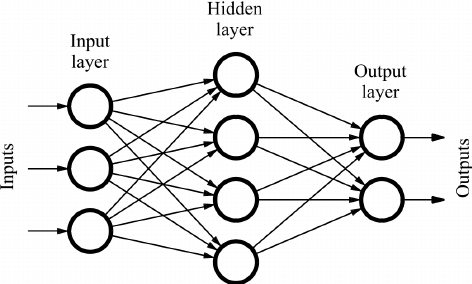
\includegraphics[width=0.9\linewidth]{Credit_Images/Sample-of-a-feed-forward-neural-network.png}
   \caption{Architecture of a generic Feedforward Neural Network \cite{inbook}.}
    \label{fig-ff-nn}
\end{figure}

\section{Why interpreting neural networks is difficult}
Neural Networks are usually treated as \emph{black boxes} of which we have little to no understanding of their inner workings. An example is present in Figure \ref{fig:panada-nn} where an adversary \cite{szegedy2014intriguing} slightly adjusted the original image on the left by generating noise which causes the Neural Network to misclassify the \emph{Panda} as a \emph{Gibbon}. From a human perspective both images are obviously of a Panda but the Neural Network was easily fooled and there is no simple way to understand why. 
\begin  {figure}[!htpb]
  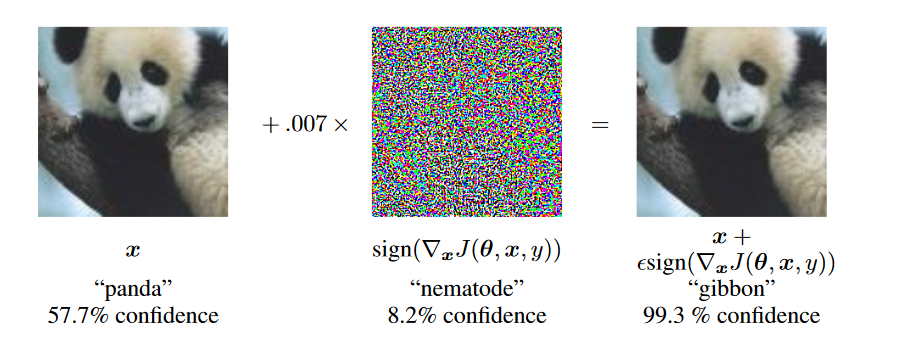
\includegraphics[width=\linewidth]{Introduction_Images/nn-unexplainable.png}
   \caption{A demonstration showing that by adding a small amount of noise to the image of a panda we were able to fool the Neural Network into misclassifying it as a gibbon \cite{goodfellow2015explaining}.}
    \label{fig:panada-nn}
\end{figure}
Looking at the architecture of a Neural Network we could identify which individual neurons activate based on the presence of certain features, an example being the shape of the pandas nose in Figure \ref{fig:panada-nn}. However, this does not seem to be true as both images contain the same features yet the Neural Network failed to correctly identify the panda. Therefore the idea of directly monitoring how neurons activate in response to features is not reliable. In the case of a linear model trained on images we could simply look at the relationship between the features extracted from algorithms such as SURF \cite{10.1016/j.cviu.2007.09.014} and SIFT \cite{Wu2013ACS} and the output. This is not as simple when working with Neural Networks due to the hidden layers having their own transformations that are learnt through backpropagating the errors \cite{10.5555/65669.104451}\cite{10.5555/525960}. In the case of a \emph{Convolutional Neural Network (CNN)} \cite{DBLP:journals/corr/Schmidhuber14} which is an image-based network, simply viewing the hidden layers may look like noise. In a CNN the features which are extracted are learnt by the network itself and may result in the reliance on noise or artifacts within the image. Another example can be seen in Figure \ref{fig:negative-nn} when changing the images to their negative the network is unable to discern the correct class. This shows that rather than specifics like edges and shapes the classifier could be relying on color specific artifacts in it's classification scheme.
\begin  {figure}[!htpb]
  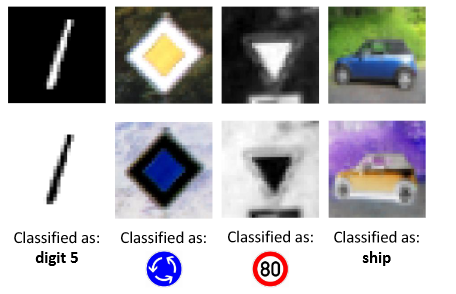
\includegraphics[width=\linewidth]{Introduction_Images/NN-negative.png}
   \caption {Simply making the images negative causes a misclassification by the network \cite{DBLP:journals/corr/HosseiniP17}.}
    \label{fig:negative-nn}
\end{figure}
It is natural to think that by providing the images altered by the noise into the training data we can prevent this form of misclassification. This is not feasible as we can not protect against every form of alteration. Therefore we need concrete explanations on how the input features affect the classification scheme of the network so that we may ascertain that the network has properly learnt actual features rather than artifacts. This extends to other network architectures. For a \emph{Recurrent Neural Network (RNN)} \cite{DBLP:journals/corr/Schmidhuber14} trained on classyfing a movie review as either good or bad, by slightly altering the input sequences it was possible to have the network misclassify 100\% of the training data \cite{DBLP:journals/corr/PapernotMSH16}. For instance changing the review “I  wouldn’t  rent  this  one  even  on  dollar  rental  night.”  into  “Excellent wouldn’t  rent  this  one  even  on  dollar  rental  night.” the network was fooled into misclassyfing the review as positive \cite{DBLP:journals/corr/PapernotMSH16}.  By simply inserting words with positive connotations into the input the RNN was mislead. The goal of providing a relationship of input features to prediction output is referred to as the \emph{attribution problem} \cite{DBLP:journals/corr/SundararajanTY17}.

\subsection{Overview of Interpretability}
As we have discussed in the previous section, linear models can be easily explained since their prediction is simply a linear combination of feature values weighted by model coefficients. However due to the need for more powerful non-linear models \emph{Random Forests} \cite{inbookb} among others  became a popular choice. Random Forests is a technique that constructs multiple decision trees and outputs the prediction as the average prediction of the individual trees. Since this technique was non-linear it was not adopted into many fields due it being difficult to interpret. A PhD thesis by \emph{Gilles Louppe} \cite{louppe2015understanding}  provided a methodology for extracting the  importance of features on a global level from Random Forests. The interpretability of Random Forests was further expanded when the popular machine learning library \emph{scikit-learn} released a blog post on how to obtain importance of features for individual predictions \cite{RandomData}. With the sudden growth in popularity of Neural Networks, interpretation was once again needed before it could replace older and weaker techniques. There have been several techniques which aim to interpret Neural Networks which range from using decision trees to approximate the network to isolating individual neurons in an attempt to explain their importance. These techniques are discussed in more detail in Chapter \ref{sect-related}. For this thesis we have chosen 2 tools which claim to be model-agnostic explainers which are explainers that can be used on any machine learning model, from linear models to neural networks and a tool which provides a deep framework to explore the inner workings of a neural network. These will be discussed in detail in Chapter \ref{sect-background}.

\section{Our approach}
\subsection{Discuss and Evaluate our chosen tools}
We discuss and evaluate 3 chosen tools which aim to provide interpretation for Neural Networks decisions. We have selected popular machine learning problems which range from the popular \emph{MNIST} digit classification problem to predicting whether a movie review posted on \emph{IMDB} is positive or negative. We have trained models with varying architectures aimed at solving these problems. Using our 3 tools we attempt to provide explanations into these models in order to discern which features have the biggest impact in determining the prediction. We also compare how these explanations differ for different input types and whether they can be easily understood.

\subsection{Generate explanations for a Neural Network used to solve a real world credit problem}
The main contribution of this work is that we apply these techniques on a real world example. The credit space is a high risk environment and therefore any machine learning technique that is used has to be interpretable. Using a credit risk dataset provided to us by Praelexis we will train both a linear model, which is a commonly used solution, and a Neural Network. Using our 2 model-agnostic tools, we will generate explanations for the Neural Network and compare them to the inherent explanations present in the linear network. Our goal is to determine whether the explanations for the neural networks are good enough to allow them to be used for risk modeling.

\section{Thesis Goals}
The goals we are aiming to achieve with this thesis are as follows:
\begin{itemize}
    \item Evaluate the provided explanations between our 3 chosen tools on various machine-learning problems.
    \item Train a linear model and a Neural Network on the provided credit risk data.
    \item Provide explanations into the credit neural network and compare the interpretability to the linear model.
    \item Answer the question whether these explanations are sufficient enough to consider Neural Networks in domains where interpretability is a strict requirement.
\end{itemize}
\section{Thesis Structure}
\begin{description}
 \item[Chapter 2] describes related techniques used for providing interpretability into Neural Networks.
 \item[Chapter 3] provides a detailed background into our 3 chosen tools by thoroughly explaining their inner workings.
 \item[Chapter 4] provides an evaluation and comparison between the explanations generated by our chosen tools on various popular machine learning problems.
 \item[Chapter 5] we train and evaluate a model trained on credit risk data and provide explanations using our tools.
 \item[Chapter 6] concludes our research.
\end{description}